\section{Generative Adversarial Networks}
\label{sec:gan}

Generative Adversarial Networks (GAN) is a framework recently proposed by Goodfellow et al which has gathered a lot of attention in the deep learning community and in the last few years many extensions have been [proposed] (citations).
GANs can be understood as a two-player game where one player is called generator $G$ playing against the discriminator $D$.
The goal of $G$ is to produce similar data to the given training set while $D$ is tasked with discriminating(?) the generated samples from the training data. Both $G$ and $D$ are learning function approximators, for example Multi-Layer Peceptron (MLP) networks as proposed in the original GAN paper.
% --> declare distribution p_data, p_model, x, z
During learning, both networks are updated in parallel according to the gradient of their respective loss function which we will explore now.\\
In the following $p_{data}$ is the true data generating distribution from which the training samples have been generated.
We don't have access to that distribution.

\subsection{Architecture}
\label{sub:gan_arch}


% http://www.slideshare.net/xavigiro/deep-learning-for-computer-vision-generative-models-and-adversarial-training-upc-2016
% TODO: recreate in tikz
\begin{figure}[htb]
\centering
  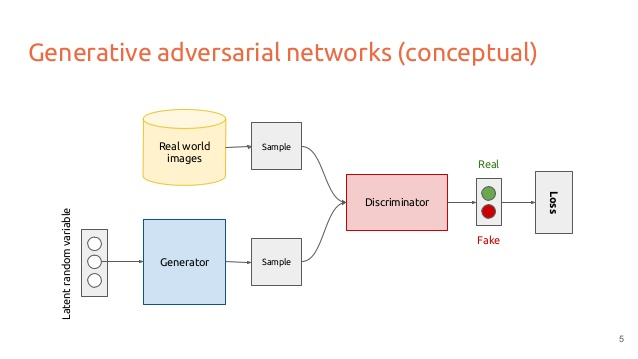
\includegraphics[width=\linewidth]{media/deep-learning-for-computer-vision-generative-models-and-adversarial-training-upc-2016-5-638.jpg}
  \caption{Conceptual idea of generative adversarial networks (source: Summer seminar UPC TelecomBCN)}\label{fig:gan_architecture}
\end{figure}


\subsubsection{Generator Network}
The generator network in the GAN framework tries to fool the discriminator $D$ by producing samples which are indistinguishable from the training data.
This process can be formally written as minimizing the following cost function.
$$
\mathcal{C}_g = \log(1 - D(G(z)))
$$
$z$ is produced by sampling from the noise prior $p_g(z)$.\\

Note that this loss function is fully differentiable which means it can be trained with backpropagation.



\subsubsection{Discriminator Network}
The objective of the discriminator network $D$ is to distinguish the generated samples produced by $G$ from the training set samples.
This process can be formalized to maximizing the cost function $\mathcal{C}_d$.
$$
\mathcal{C}_d = \log\big(\log D(x) + \log (1 - D(G(z))\big)
$$



\subsection{Training}
\label{sub:gan_training}
The GAN framework can be fully trained with stochastic backpropagation due to both $D$ and $G$ being differentiable.

Combining the cost functions of generator and discriminator yield us the following objective with value function $V(G,D)$.
$$
\min_G \max_D V(D,G) = \mathbb{E}_{x \sim p_{data}}[\log D(x)] + \mathbb{E}_{z \sim p_z(z)}[\log(1 - D(G(z)))]
$$
In the original GAN paper an minibatch-based algorithm for training GAN is proposed, but we will take a look at an the online learning version below:\\
\begin{algorithm}
  \caption{Online learning of generative adversarial networks $-$ simple version ($k=1$)}
  \label{alg:gan_online}
  \begin{algorithmic}[1]
    \Let{$\eta_d, \eta_g$}{Learning rate of discriminator and generator networks, respectively}
    \Let{$\theta_d, \theta_g$}{Parameters of function approximators}
    \For{number of training iterations}
      \Let{$z_d$}{sample from noise prior $p_g(z)$}
      \Let{$z_g$}{sample from noise prior $p_g(z)$}
      \Let{$x$}{example from training set}
      \Let{$\theta_d$}{$\theta_d + \eta_d \nabla_{\theta_d} \bigg[\log D(x) + \log \big(1 - D(G(z_d))\big)\bigg]$}
      \Let{$\theta_g$}{$\theta_g - \eta_g \nabla_{\theta_g} \bigg[\log\big(1 - D(G(z_d))\big)\bigg]$}
    \EndFor
  \end{algorithmic}
\end{algorithm}

In algorithm \ref{alg:gan_online} the original algorithm has been modified for single pass (online) learning.
Sampling minibatches from the noise prior and $p_{data}(x)$ result in the minibatch version.
Additionally, it is often required for practical reasons to let the discriminator run multiple backward passes while updating the generator once (why?).
Note that the discriminator will ascend while the generator descend its gradient due to maximizing $\mathcal{C}_d$ but minimizing $\mathcal{C}_g$ (correct?).

\subsection{Stability and Performance}
\label{sub:gan_stability}
In the practical case where both function approximators $G$ and $D$ are represented using a neural network,
GANs have been shown to be difficult to train using gradient descent.
These issues have been credited to the problem of finding the nash equilibrium in the minimax-game with continious, high-dimensional parameters whereas current gradient-based methods are [designed] to reach an minimum.
Additionally to these hypothetical thoughts, \cite{gan_distinguish_crit:2014} have shown that these methods may fail to converge.
Acknoledging these problems, Salimans et al \cite{improved_gan:2016} has studied the stability and performance of GAN in detail resulting in a number of practical methods improving sample generation and improved semi-supervised learning performance.
We will take a look at a selection of these methods in the following, focussing on neural networks as approximators.

\subsubsection{Freeze Learning}
\label{ssub:gan_freeze_learning}
One of the main issues prominent during early GAN research is the disparity between $G$ and $D$.
Commonly during training one of these networks will outpace the other resulting in degraded gradients where the other player is unable to learn from.
Freeze learning is one of the natural counter to this problem, just freezing either $G$ or $D$ until the other network has catched up (formulation!).
In practice the generator is far slower to train than the discriminator in most cases (citation).


\subsubsection{Label Smoothing}
\label{ssub:gan_label_smoothing}
Another basic idea to improve gradient flow is to replace the binary classification values $0/1$ with smoothed values $0.1/0.9$ or $\epsilon/1-\epsilon$.
This guarantees to provide the generator with an informative gradient to improve learning performance
Additionally, smoothed labels have been shown to reduce the attack surface of neural networks to adversarial examples \cite{adv_examples:2016}.
% TODO replace 0/1 with e/1 − e ??
% TODO one-sided label smoothing


\subsubsection{Feature Matching}
\label{ssub:gan_feature_matching}

\subsubsection{Minibatch discrimination}
\label{ssub:gan_minibatch_discrimination}

\subsubsection{Historical Averaging}
\label{ssub:gan_historical_averaging}




\subsubsection{Normalizing Flows}
\label{ssub:gan_nf}









\subsection{Application}
\label{sub:gan_application}
GAN have been applied to many different areas which include generating images (GAN, DCGAN, LAPGAN), sequences (SeqGAN), videos (\cite{gan_video:2016}), 3D objects (\cite{gan_3d:2016}), text-to-image synthesis (\cite{gan_t2i:2016})
\subsection{Extensions}
\label{sub:gan_extensions}

\subsubsection{LAPGAN}
\label{ssub:lapgan}

\subsubsection{DCGAN}
\label{ssub:dcgan}


